% ----------------------------------------------------------------------------------------------------- %
% Apêndice 
% ----------------------------------------------------------------------------------------------------- %
\chapter{Apêndice}
\label{cap:apendice}

\section*{Apêndice I}

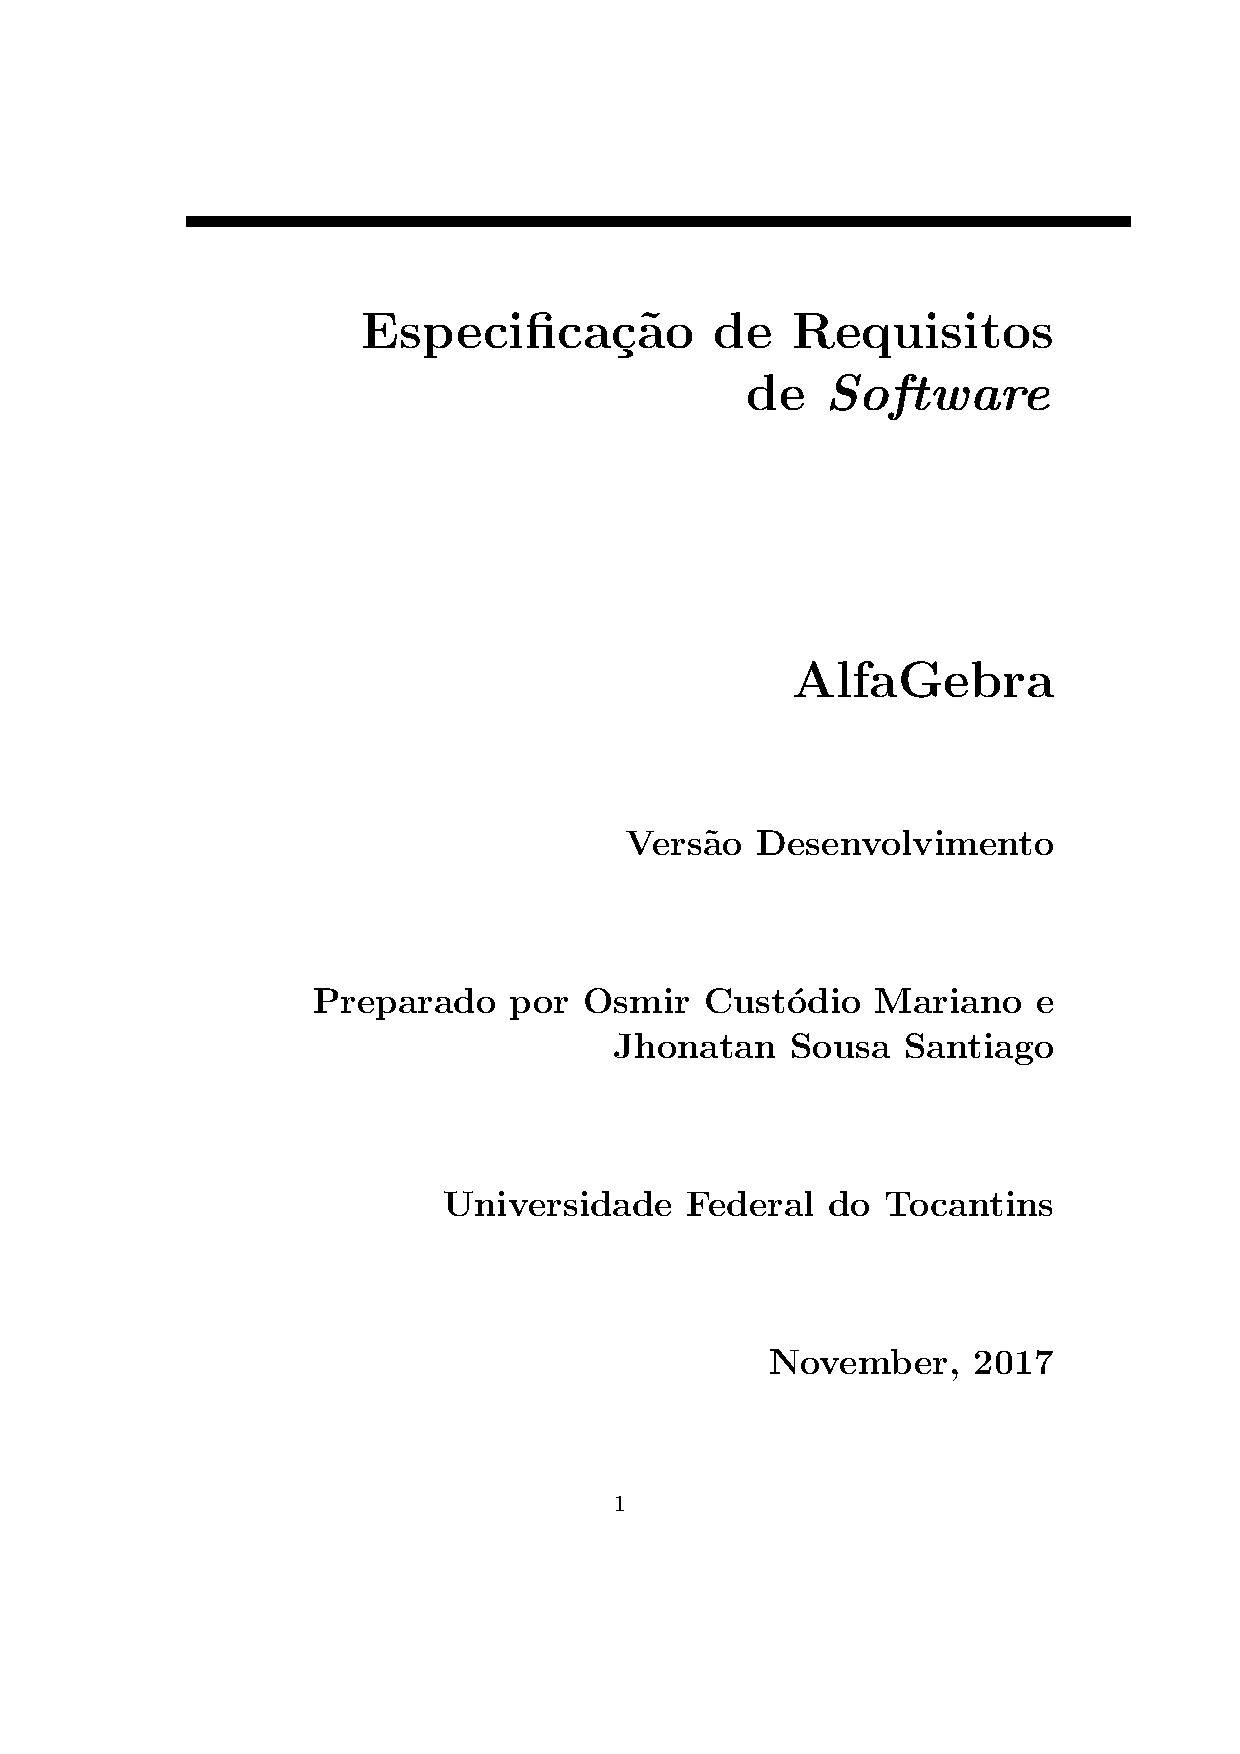
\includepdf[pages=-]{Arquivos/especifi_requisitos.pdf}

\section*{Apêndice II}
\subsection*{Formulário de avaliação de desempenho}
\label{questionario_base}

\begin{enumerate}
    \item Qual foi a sua maior dificuldade com a disciplina? 
    
(   ) Falta de tempo para dedicação ao estudo\\
(   ) Falta de clareza do professor\\
(   ) Desprovimento de disciplinas pré-requisitos \\
(   ) Falta de interação com professor\\
(   ) Alto nível de abstração da disciplina\\
(   ) Não consegui entender a matéria\\
(   ) Outras

    \item Por quantas vezes já está cursando a disciplina?

(   )  1 vez\\
(   )  2 vezes\\
(   )  3 ou mais

    \item Qual o método de estudo utilizado?
    
(   ) Estudo em grupo\\
(   ) Estudo através de listas de exercícios\\
(   ) Sanar dúvidas em atendimentos com professor\\
(   ) Estudo individual\\
(   ) Estudo através de livros\\
(   ) Sanar dúvidas na sala de aula\\
(   ) Outros

\item Se fosse disponibilizado algum recurso tecnológico para auxiliar no estudo/aprendizagem da álgebra linear, você usaria?

(   ) Sim\\
(   ) Não\\
(   ) Talvez

\item O que você achou da ideia de um recurso tecnológico para auxiliar no estudo/aprendizado?

(   ) Excelente\\
(   ) Boa\\
(   ) Razoável\\
(   ) Ruim\\
(   ) Péssima
	
\item Quais conteúdos gostaria que fossem abordados nesses recursos tecnológico? OBS: Pode marcar mais de um item.

(  ) Sistemas de equações Lineares\\
(  ) Espaços Vetoriais\\
(  ) Transformações lineares
	
\item Como você classifica seu aprendizado na disciplina de Álgebra Linear até o presente momento?

(   ) Excelente\\
(   ) Bom\\
(   ) Regular\\
(   ) Ruim\\
(   ) Péssimo

\item Em relação ao seu curso, você considera que essa disciplina é:

(   ) Importante\\
(   ) Tem alguma importância\\
(   ) Pouco importante

\item Qual o grau de dificuldade da disciplina?

(   ) Alto\\
(   ) Médio\\
(   ) Razoável\\
(   ) Fácil

\item Com que frequência você procura o professor(a) (fora da aula) para tirar suas dúvidas?

(   ) Muita frequência\\
(   ) Razoável\\
(   ) Poucas\\
(   ) Nunca procurei

\item Após cursar a disciplina, seu interesse pelo assunto aumentou? (Para aqueles que já cursaram mais de um vez a disciplina)

(   ) Sim\\
(   ) Não

\item Cite um ou mais pontos fortes da disciplina.

\_\_\_\_\_\_\_\_\_\_\_\_\_\_\_\_\_\_\_\_\_\_\_\_\_\_\_\_\_\_\_\_\_\_\_\_\_\_\_\_\_\_\_\_\_\_\_\_\_\_\_\_\_\_\_\_\_\_\_\_\_\_\_\_\_\_\_\_\_\_\_\_\_\_\_\_\_\_\_\_\_\_\_\_\_\_\_\_\_\_\_\_\_\_\_\_\_\_\_\_\_\_\_\_\_\_\_\_\_\_\_\_\_\_\_\_\_\_\_\_\_\_\_\_\_\_\_\_\_\_\_\_\_\_\_\_\_\_\_\_\_\_\_\_\_\_\_\_\_\_\_\_\_\_\_\_\_\_\_\_\_\_\_\_\_\_\_\_\_\_\_\_\_\_\_\_

\item Que sugestões você daria para melhorar a disciplina?

\_\_\_\_\_\_\_\_\_\_\_\_\_\_\_\_\_\_\_\_\_\_\_\_\_\_\_\_\_\_\_\_\_\_\_\_\_\_\_\_\_\_\_\_\_\_\_\_\_\_\_\_\_\_\_\_\_\_\_\_\_\_\_\_\_\_\_\_\_\_\_\_\_\_\_\_\_\_\_\_\_\_\_\_\_\_\_\_\_\_\_\_\_\_\_\_\_\_\_\_\_\_\_\_\_\_\_\_\_\_\_\_\_\_\_\_\_\_\_\_\_\_\_\_\_\_\_\_\_\_\_\_\_\_\_\_\_\_\_\_\_\_\_\_\_\_\_\_\_\_\_\_\_\_\_\_\_\_\_\_\_\_\_\_\_\_\_\_\_\_\_\_\_\_\_\_

\item Quais suas dificuldades ao estudar álgebra linear?

\_\_\_\_\_\_\_\_\_\_\_\_\_\_\_\_\_\_\_\_\_\_\_\_\_\_\_\_\_\_\_\_\_\_\_\_\_\_\_\_\_\_\_\_\_\_\_\_\_\_\_\_\_\_\_\_\_\_\_\_\_\_\_\_\_\_\_\_\_\_\_\_\_\_\_\_\_\_\_\_\_\_\_\_\_\_\_\_\_\_\_\_\_\_\_\_\_\_\_\_\_\_\_\_\_\_\_\_\_\_\_\_\_\_\_\_\_\_\_\_\_\_\_\_\_\_\_\_\_\_\_\_\_\_\_\_\_\_\_\_\_\_\_\_\_\_\_\_\_\_\_\_\_\_\_\_\_\_\_\_\_\_\_\_\_\_\_\_\_\_\_\_\_\_\_\_

\item O que você considera mais difícil na álgebra Linear? 

\_\_\_\_\_\_\_\_\_\_\_\_\_\_\_\_\_\_\_\_\_\_\_\_\_\_\_\_\_\_\_\_\_\_\_\_\_\_\_\_\_\_\_\_\_\_\_\_\_\_\_\_\_\_\_\_\_\_\_\_\_\_\_\_\_\_\_\_\_\_\_\_\_\_\_\_\_\_\_\_\_\_\_\_\_\_\_\_\_\_\_\_\_\_\_\_\_\_\_\_\_\_\_\_\_\_\_\_\_\_\_\_\_\_\_\_\_\_\_\_\_\_\_\_\_\_\_\_\_\_\_\_\_\_\_\_\_\_\_\_\_\_\_\_\_\_\_\_\_\_\_\_\_\_\_\_\_\_\_\_\_\_\_\_\_\_\_\_\_\_\_\_\_\_\_\_

\item Você conhece ou já fez uso de algum sistema que te auxiliou no estudo da álgebra linear? 

\_\_\_\_\_\_\_\_\_\_\_\_\_\_\_\_\_\_\_\_\_\_\_\_\_\_\_\_\_\_\_\_\_\_\_\_\_\_\_\_\_\_\_\_\_\_\_\_\_\_\_\_\_\_\_\_\_\_\_\_\_\_\_\_\_\_\_\_\_\_\_\_\_\_\_\_\_\_\_\_\_\_\_\_\_\_\_

\item Se sim, qual(is)?

\_\_\_\_\_\_\_\_\_\_\_\_\_\_\_\_\_\_\_\_\_\_\_\_\_\_\_\_\_\_\_\_\_\_\_\_\_\_\_\_\_\_\_\_\_\_\_\_\_\_\_\_\_\_\_\_\_\_\_\_\_\_\_\_\_\_\_\_\_\_\_\_\_\_\_\_\_\_\_\_\_\_\_\_\_\_\_\_\_\_\_\_\_\_\_\_\_\_\_\_\_\_\_\_\_\_\_\_\_\_\_\_\_\_\_\_\_\_\_\_\_\_\_\_\_\_\_\_\_\_\_\_\_\_\_\_\_\_\_\_\_\_\_\_\_\_\_\_\_\_\_\_\_\_\_\_\_\_\_\_\_\_\_\_\_\_\_\_\_\_\_\_\_\_\_\_

\item Quais os recursos (seja eles tecnológicos ou não) que o seu professor utilizou para o ensino da disciplina?

\_\_\_\_\_\_\_\_\_\_\_\_\_\_\_\_\_\_\_\_\_\_\_\_\_\_\_\_\_\_\_\_\_\_\_\_\_\_\_\_\_\_\_\_\_\_\_\_\_\_\_\_\_\_\_\_\_\_\_\_\_\_\_\_\_\_\_\_\_\_\_\_\_\_\_\_\_\_\_\_\_\_\_\_\_\_\_\_\_\_\_\_\_\_\_\_\_\_\_\_\_\_\_\_\_\_\_\_\_\_\_\_\_\_\_\_\_\_\_\_\_\_\_\_\_\_\_\_\_\_\_\_\_\_\_\_\_\_\_\_\_\_\_\_\_\_\_\_\_\_\_\_\_\_\_\_\_\_\_\_\_\_\_\_\_\_\_\_\_\_\_\_\_\_\_\_

\item Se fosse desenvolvido um sistema para auxiliar você aluno, no aprendizado da Álgebra Linear, a qual esse apresentaria um tutorial dos principais conteúdos da Álgebra e opção em que o aluno entre com a expressão e o sistema mostre o passa-a-passo da resolução. Marque o quanto ele ajudaria?

(   ) Ajudaria muito\\
(   ) Ajudaria, mas prefiro não utilizar\\
(   ) Ajudaria Pouco\\
(   ) Não ajudaria 

\item Em sua opinião a utilização desse sistema durante as aulas ou fora possibilitará mais dinamismo e aprendizado da matéria?

(   ) Sim\\
(   ) Não\\
(   ) Não sei

\end{enumerate}



